\documentclass[a4paper,12pt]{article}
%\documentclass[a4paper,12pt]{scrartcl}

\usepackage[utf8]{inputenc}
\usepackage{amsmath}
\usepackage{graphicx}
\usepackage{listings}

\title{}
\author{}
\date{}
\def\BibTeX{{\rm B\kern-.05em{\sc i\kern-.025em b}\kern-.08em
    T\kern-.1667em\lower.7ex\hbox{E}\kern-.125emX}}
\pdfinfo{%
  /Title    (Messwerterfassung und regenerative Energieerzeugung)
  /Author   (Marcel Hanke,)
  /Creator  ()
  /Producer ()
  /Subject  ()
  /Keywords ()
}

\begin{document}
\maketitle

\section{Literaturrecherche}
\subsection{Wie funktioniert die Gewinnung elektrischer Energie mit Hilfe von Photovoltaik?}
Wie funktioniert die Gewinnung elektrischer Energie mit Hilfe von Photovoltaik?\\
Um eine Gewinnung elektrischer Energie mithilfe von Photovoltaik zu ermöglichen, braucht es unter anderem eine Solarzelle. Betrachten wir zum einfacheren Verständnis eine Photodiode, die in ihrer Wirkungsweise einer Solarzelle gleichkommt. 
Die Grundlage für die Photovoltaiktechnik liefert uns das zweite Bohrsche Postulat: "Der Übergang eines Elektrons von einer Schale zur anderen erfolgt unter Emission oder Absorption von elektromagnetischer Strahlung." Sprich: Trifft Licht auf ein Elektron, so wird dieses auf ein anderes Energieniveau angehoben. 

Stellen wir uns die Photodiode so vor, als bestünde sie aus zwei aneinandergesetzten Kristallen. Der eine n-dotiert (Elektronenüberschuss) und der andere p-dotiert (Elektronenmangel). Fügt man diese nun zusammen, so entsteht ein Gleichgewicht am Übergang, denn die überschüssigen Elektronen werden von den "Elektronenlöchern" im p-dotierten Teil angezogen. Zurück bleibt eine ortsfeste positive Ladung im n-dotierten Raum und eine ortsfeste negative Ladung im p-dotierten Raum. Diesen Ausgleich bezeichnet man elektrisches Feld. Durch die steigende Anzahl an ortsfesten Ladungen entsteht der sog. Diffusionsstrom. Dieser Strom und das el. Feld heben sich gegenseitig auf.
Durch das einfallende Licht werden nun die Elektronen im el. Feld zur n-dotierten Seite befördert. Bringt man jeweils einen Kontakt an die n-und p-dotierte Seite, lässt sich der sog. Photostrom abgreifen. 
\subsection{Was versteht man unter dem Maximum-Power-Point (MPP) einer Solarzelle?}
Der Punkt unter welchem die Solarzelle bei der aktueller Bestrahlung und Temperatur die Maximale Leistung abgibt. Da die Leistung das Produkt aus der Spannung U und dem Strom I ist, lässt sich aus der grafischen Darstellung der MMP als die größtmögliche Fläche unter dem Grafen der Leistung darstellen. Um diesen Punkt möglichst optimal zu treffen muss entweder die Stromstärke oder die Spannung welche an der Solarzelle anliegt korrigiert werden.

\subsection{Welche Möglichkeiten zur Speicherung von (regenerativ erzeugter) elektrischer Energie gibt es?}
Hier gibt es eine viel Zahl an Möglichkeiten (vier in zunehmender Kapazität):
\begin{itemize}
 \item Kondensator
 \item Batterien/Akkus (Chemischer Prozess)
 \item Elektrolyse/Brennstoffzelle (Wasserstoffspeicherung)
 \item Wasserspeicherkraftwerke 
\end{itemize}


\section{Bestimmung des Maximum-Power-Points}
Bei der Bestimmung des Maximum-Power-Points (im weiteren Dokument MPP genannt) kommt folgende Formel zu Berechnung der Leistung zum Einsatz:\newline
\large \begin{center}
        $P = \frac{U^2}{R}$
       \end{center}
\small \begin{itemize}
    \item P = Power = Leistung (in Watt)
    \item U = Spannung (in Volt)
    \item R = Wiederstand (in Ohm)
\end{itemize} 
\normalsize Die erste Lichtquelle ist eine 200W Glühbirne, hier wurden folgende Spannungen gemessen:\newline
 \begin{tabular}{ll}
  \textbf{Wiederstand} & \textbf{Stannung} \\
  100 $ \Omega $ & 0,516 V \\
  220 $ \Omega $ & 1,160 V \\
  270 $ \Omega $ & 1,547 V \\
  470 $ \Omega $ & 2,578 V \\
  1,2 k$ \Omega $ & 4,770 V \\
  8,2 k$ \Omega $ & 5,285 V \\
  10 k$ \Omega $ & 5,543 V \\
  68 k$ \Omega $ & 5,414 V \\
  100 k$ \Omega $ & 5,414 V \\
  1 M$ \Omega $ & 5,414 V \\
 \end{tabular}

Nach der Berechnung der Leistung erhalten wir folgende Kurve und ein MMP von 0,01896 W:\newline
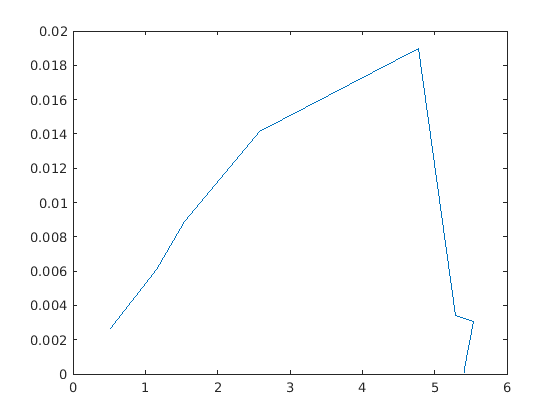
\includegraphics{200WGB}
\newline \newline
Die zweite Lichtquelle ist eine 60W Glühbirne und hier erhalten wir die folgende Werte:\newline
 \begin{tabular}{ll}
  \textbf{Wiederstand} & \textbf{Stannung} \\
  100 $ \Omega $ & 0 V\\
  220 $ \Omega $ & 0,129 V\\
  270 $ \Omega $ & 0,129 V\\
  470 $ \Omega $ & 0,387 V\\
  1,2 k$ \Omega $ & 1,031 V\\
  8,2 k$ \Omega $ & 4,254 V \\
  10 k$ \Omega $ & 4,512 V \\
  68 k$ \Omega $ & 4,641 V \\
  100 k$ \Omega $ & 4,641 V \\
  1 M$ \Omega $ & 4,641 V \\
 \end{tabular}
Nach der Berechnung der Leistung erhalten wir folgende Kurve und ein MMP von 0,002207 W:\newline
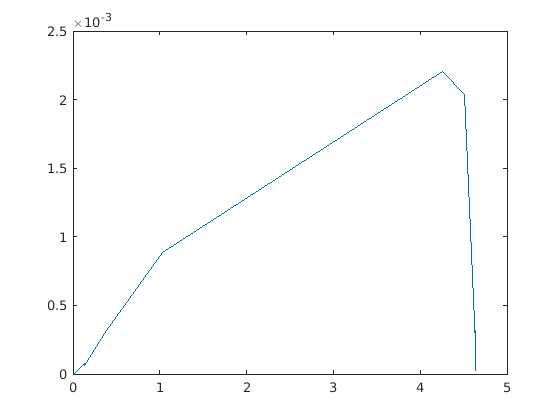
\includegraphics{60WGB}
\newline \newline
Die dritte Lichtquelle sind drei 15W Leuchtstoffröhren und hier erhalten wir die folgende Werte:\newline
 \begin{tabular}{ll}
  \textbf{Wiederstand} & \textbf{Stannung} \\
  100 $ \Omega $ & 0.002\\
  220 $ \Omega $ & 0.081 V\\
  270 $ \Omega $ & 0.105 V\\
  470 $ \Omega $ & 0.164 V\\
  1,2 k$ \Omega $ & 0.429 V\\
  8,2 k$ \Omega $ & 2.642 V \\
  10 k$ \Omega $ & 2.503 V \\
  68 k$ \Omega $ & 4.198 V \\
  100 k$ \Omega $ & 4.247 V \\
  1 M$ \Omega $ & 4.337 V \\
 \end{tabular}
Nach der Berechnung der Leistung erhalten wir folgende Kurve und ein MMP von 0,00085 W:\newline
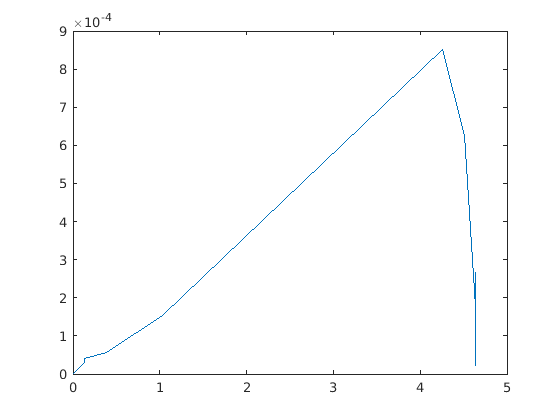
\includegraphics{OSRAML6W640}
\newline \newline

\subsection{Solare Wechselrichter}
In SolarenWechselrichtern sind MPP-Tracker installiert, welche eine Regelung zur maximalen Leistungsausbeute ermöglichen. Dies ist nötig, da die Solarzelle bei unterschiedlichen Bestrahlungstärken unterschiedliche optimale Betriebspunkte besitzt.
Das Vorgehen ist hier wie folgt:
\begin{enumerate}
 \item Speichern der aktuellen Leistung
 \item Änderung der Steuergröße
 \item kleine Pause
 \item Vergleich der Leistung mit der zuvor gemessenen, wenn die Aktuelle größer ist, wird diese gespeichert
 \item Korrektur der Steuergröße
 \item Fortfahren mit Punkt 3
\end{enumerate}
~\cite{MPPT}

\section{Energiespeicherung}
Der Kondensator besteht auf 3 Elementen, zwei Elektroden und einem Dielektikum. Wenn nun Spannung an den Kondensator angelegt wird, entsteht ein elektrisches Feld. Dieses Feld wird nach dem abschalten der Spannungsquelle wieder zu Strom "gewandelt" und fließt zurück in den Stromkreis. \\
Unser Kondensator besitzt eine Kapazität von 1 F (Farad) und unser Wiederstand beträgt 1k $\Omega$. Da die Aufladezeit $\tau$ nur von Kapazität C und Wiederstand R abhängt, erhalten wir\\
\large \begin{center}
       $$ \tau = R_{\mathrm{C}} \cdot C $$ \end{center}\\
\normalsize In unserem Fall folgendes ergibt:\newline
\large \begin{center}$ \tau = 1 k \Omega * 1000000 \mu F  = 16,66 min$\end{center}\\

\bibliography{verzeichnis1}
\bibliographystyle{plain}

\appendix
\section{Leistungsskript zu 2.2}
\lstinputlisting{Leistungsscript.m}

\end{document}
